\chapter{Theoretical Motivation} \label{chap-theory}

DGLAP
Higgs related to top
interaction lagrangian with effective operators
electric dipole moment and a top quark with 4/3 charge
anomolous couplings
talk about top quarks - different chapter maybe?

\section{The Standard Model of Particle Physics} \label{sec-StandardModel}

\begin{equation}
SU(3)_C \times SU(2)_L \times U(1)_Y
\end{equation}

\subsection{The Electroweak Theory} \label{subsec-ElectroweakTheory}

\subsection{Quantum Chromodynamics} \label{subsec-QuantumChromodynamics}

\begin{equation} \label{equ-ckm}
\begin{pmatrix}
d' \\
s' \\
b' 
\end{pmatrix}
=
\begin{pmatrix}
V_{ud} & V_{us} & V_{ub} \\
V_{cd} & V_{cs} & V_{cb} \\
V_{td} & V_{ts} & V_{tb} 
\end{pmatrix}
\begin{pmatrix}
d \\
s \\
b 
\end{pmatrix}
\end{equation}

\subsection{Electroweak Symmetry Breaking} \label{subsec-ElectroweakSymmetryBreaking}

\begin{figure}
\begin{center}
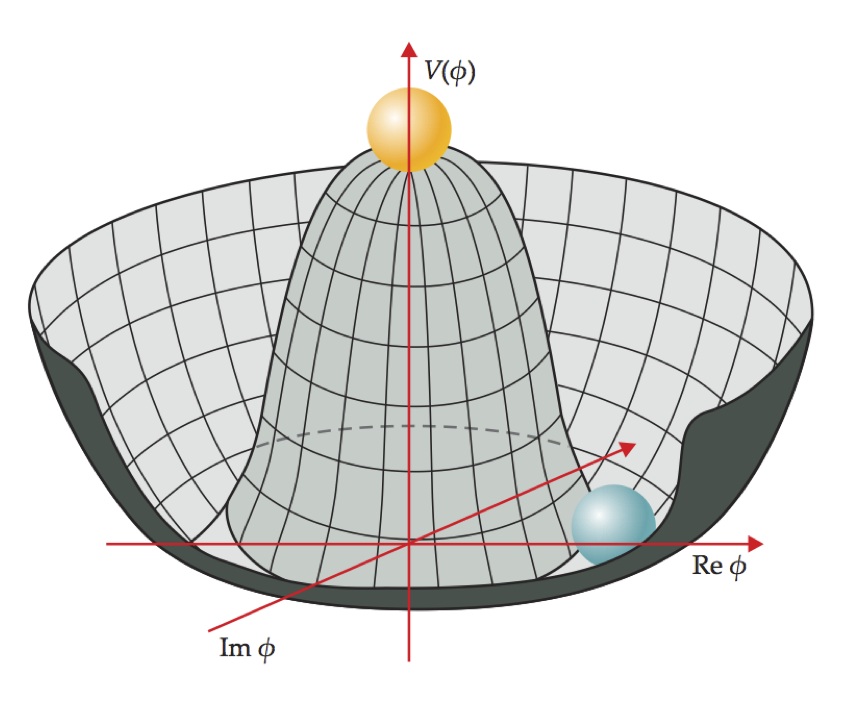
\includegraphics[width=0.7\textwidth]{Figures/MexicanHatPotential.png}
\caption{The ``Mexican Hat Potential" describing the vacuum expectation value of the Higgs in the real and imaginary planes, such that the minima lies below zero.}
\end{center}
\end{figure}

\begin{figure}
\begin{center}
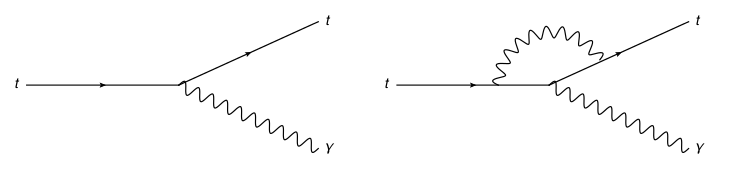
\includegraphics[width=\textwidth]{Figures/TopPhotonVertex.png}
\caption{Top-photon vertex. Left: Leading Order (LO). Right: One-Loop correction (NLO).}
\end{center}
\end{figure}

\begin{equation} \label{eqn-interactionlagrangian}
\lumi_{\gamma t\bar{t}} = -eQ_t\bar{t}\gamma^{\mu}tA_{\mu} - e\bar{t}\frac{i\sigma^{\mu\nu}q_{\nu}}{m_t}(d^{\gamma}_V+id^{\gamma}_A\gamma^5)tA_{\mu}
\end{equation}

\begin{equation}
\lumi^{eff.} = \Sum \frac{C_x}{\Lambda_x}O_x + ... ,
\end{equation}

\begin{align}\label{eqn-smparameterisations}
\delta d^{\gamma}_V = \frac{\sqrt{2}}{e}\text{Re}[c_WC^{33}_{uB\phi} + s_WC^{33}_{uW}]\frac{vm_t}{\Lamdba^2} \\
\delta d^{\gamma}_A = \frac{\sqrt{2}}{e}\text{Im}[c_WC^{33}_{uB\phi} + s_WC^{33}_{uW}]\frac{vm_t}{\Lamdba^2}
\end{align}

\begin{figure}
\begin{center}
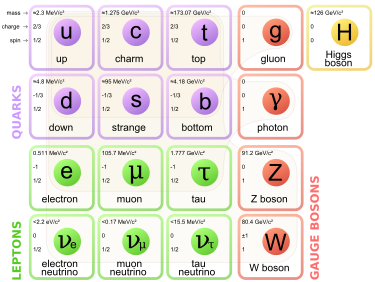
\includegraphics[width=0.8\textwidth]{Figures/StandardModel.png}
\caption{The Standard Model of particle physics.}
\end{center}
\end{figure}

\section{The Top Quark} \label{sec-TheTopQuark}

\begin{figure} \label{fig-ttbarProductionLHC}
\begin{center}
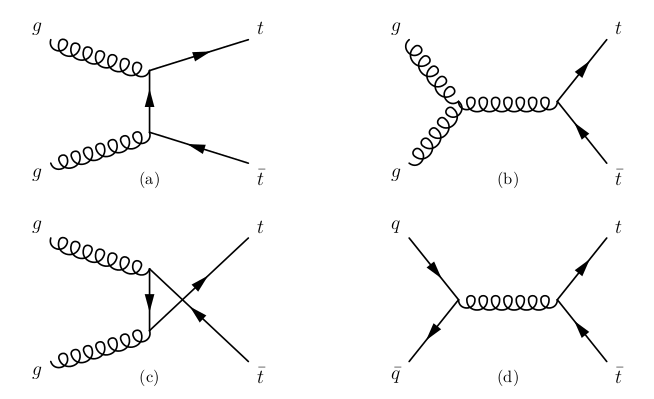
\includegraphics[width=\textwidth]{Figures/ttbarProductionLHC.png}
\caption{Lowest level diagrams for $t\bar{t}$ production at the LHC. Gluon scattering processes, {(a)}, {(b)}, and {(c)}, are the dominant processes at LHC energies, while quark scattering, process {(d)}, is the dominant one at TeVatron energies. \cite{SergeyThesis}}
\end{center}
\end{figure}

\begin{figure} \label{fig-singletopProductionLHC}
\begin{center}
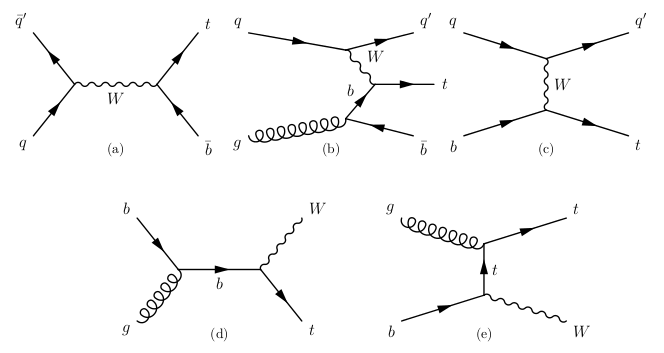
\includegraphics[width=\textwidth]{Figures/singletopProductionLHC.png}
\caption{Leading-order level diagrams for single top production at the LHC. {(a)} s-channel, {(b)} and {(c)} represent the t-channel, {(d)} and {(e)} both represent the two tW channels. \cite{SergeyThesis}}
\end{center}
\end{figure}

\begin{figure}
\begin{center}
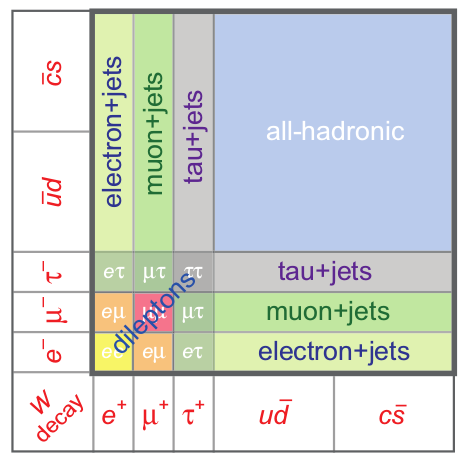
\includegraphics[width=0.5\textwidth]{Figures/ttbarDecayFractions.png}
\caption{Branching fractions of the W decays within top quark pairs. \cite{ttbarDecayFractions}}
\end{center}
\end{figure}

\begin{figure} \label{fig-ttgammaFeynmanDiagram}
\begin{center}
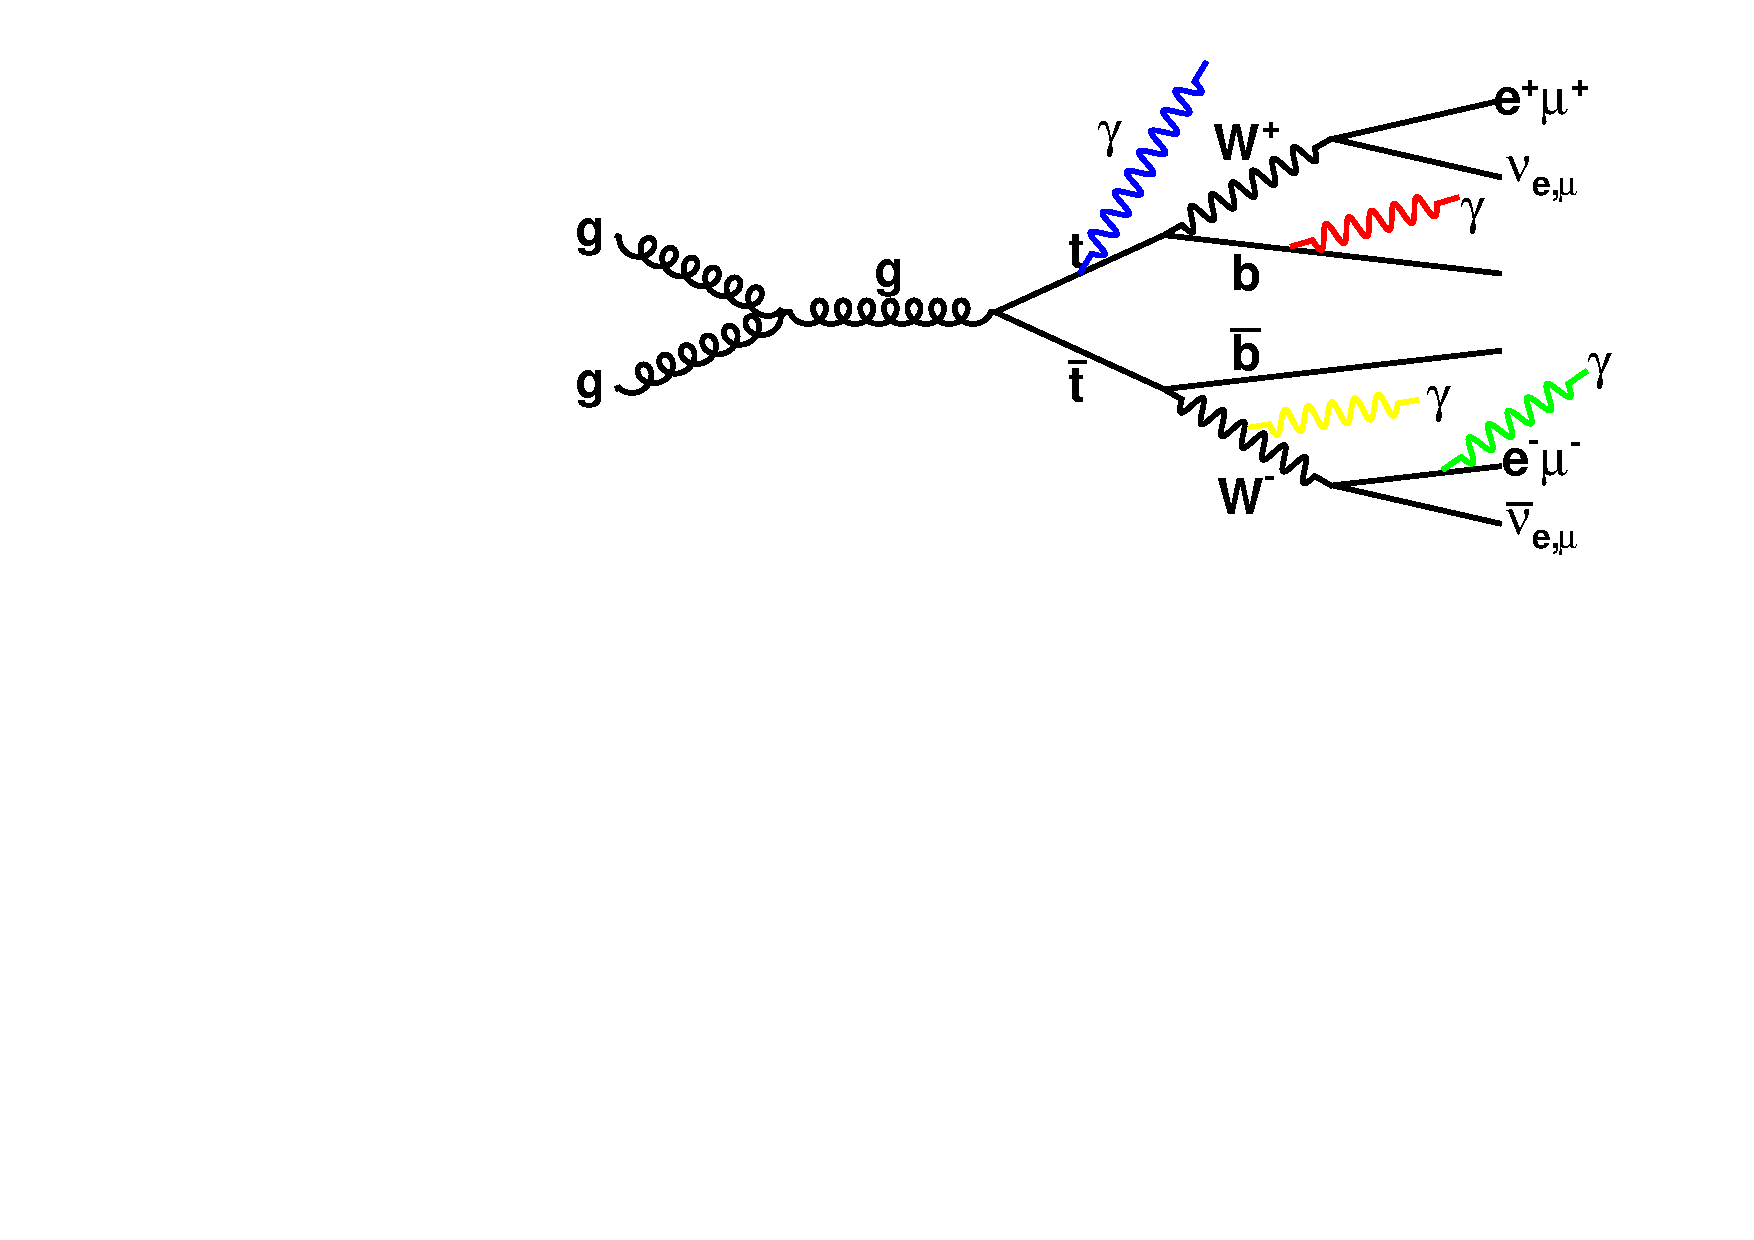
\includegraphics[width=0.9\textwidth]{Figures/ttgammaFeynmanDiagram.pdf}
\caption{}
\end{center}
\end{figure}